\begin{knitrout}
\definecolor{shadecolor}{rgb}{0.969, 0.969, 0.969}\color{fgcolor}\begin{figure}

{\centering 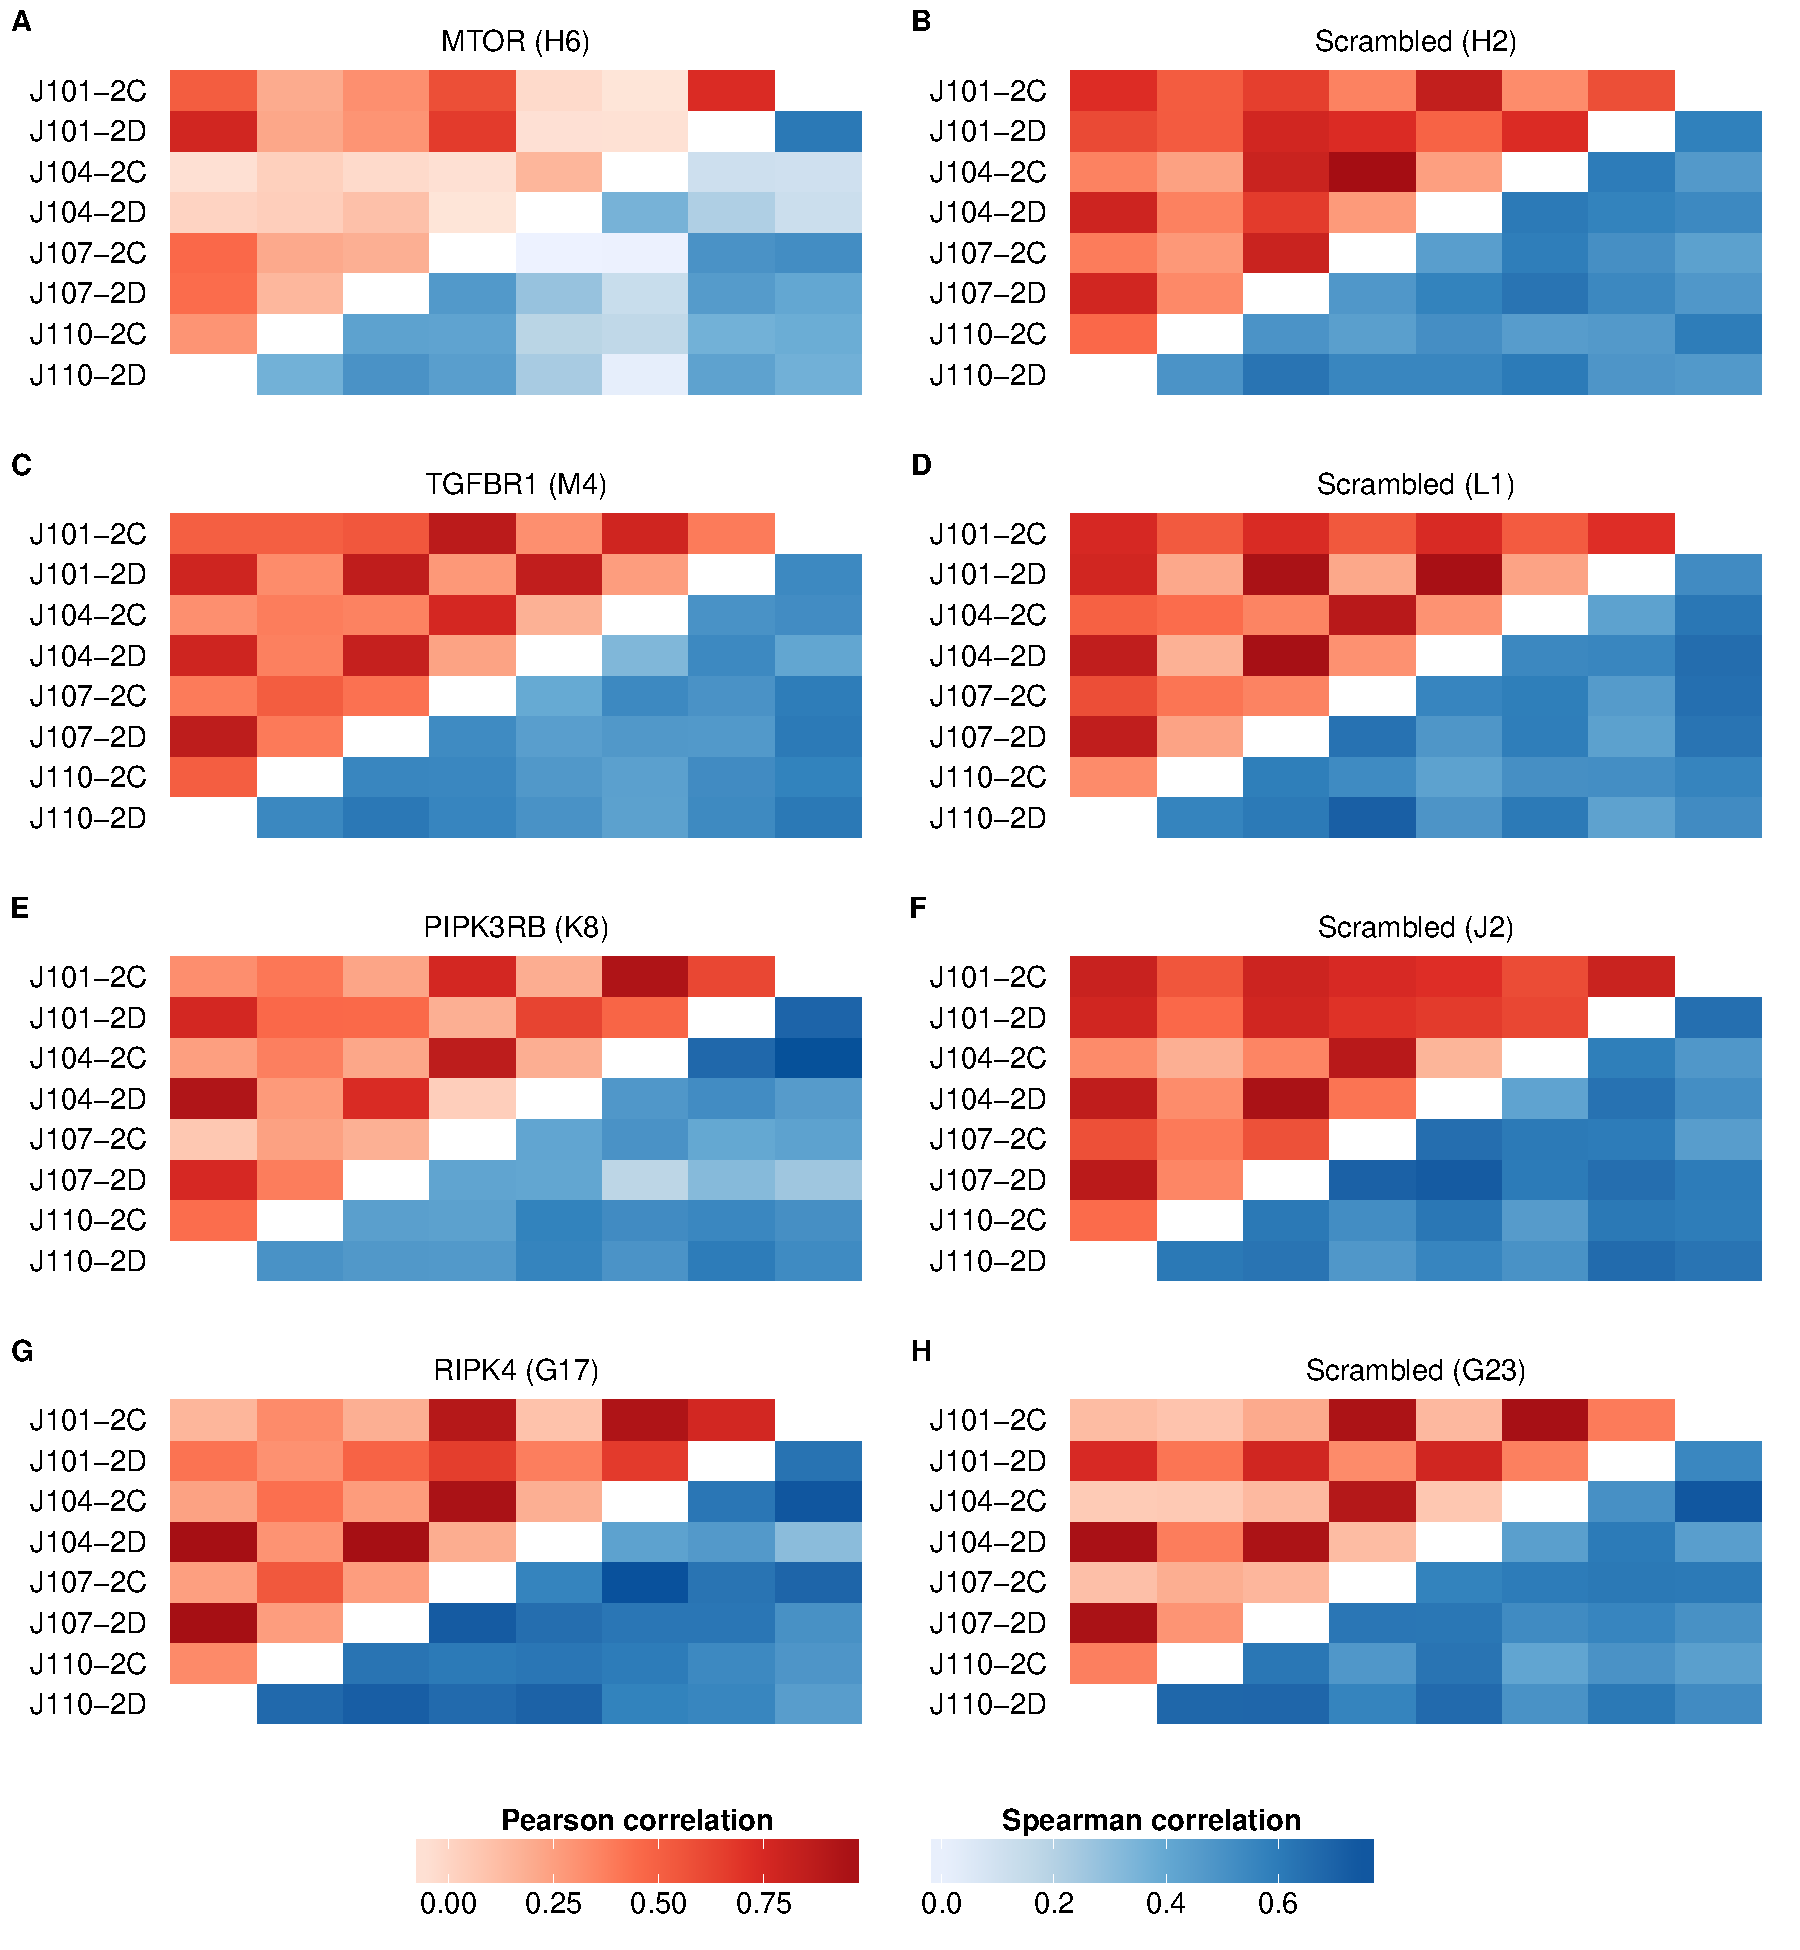
\includegraphics[width=\maxwidth]{figures/R/forest-corr-forest-corr-1} 

}

\caption[Heatmap representations of Pearson and Spearman correlation between feature importance scores from random forest analysis.]{Heatmap representations of correlation matrices obtained by comparing importance scores of features as determined by random forest analysis. Red shades indicate Pearson's product-moment correlation while blue shades visualize Spearman's rank correlation coefficients. For each gene and scrambled well, all available 8 replicates of the \textit{Brucella} Dharmacon unpooled dataset were considered.}\label{fig:forest-corr}
\end{figure}


\end{knitrout}

